\documentclass[12pt,a4paper]{article}
\usepackage[utf8]{inputenc}
\usepackage{amsmath}
\usepackage{amsfonts}
\usepackage{amssymb}
\usepackage{graphicx}
\author{José Antonio García Hernández}
\title{The Heatbath algorithm}
\newcommand*{\eps}{0.05}
\newcommand*{\Real}{\text{Re}\,}
\usepackage{tikz}
\usepackage{pgfplots}
\pgfplotsset{compat=newest}

\begin{document}
\maketitle
In Yang Mills theories, Heatbath algorithms generate updates for a variable $U_{\mu}(x)$ with probability density
\begin{equation}    
    dP(U) \propto \exp(-S[U])dU,
\end{equation}
where $S[U]$ is the action of the configuration $[U]$.

Let's define the sum of staples
\begin{equation}
    \Sigma_{\mu}(x) = \sum_{\nu\ne\mu} [U_{\nu}(x)U_{\mu}(a+\hat\nu)U^{\dagger}_{\nu}(x+a\hat\mu) + U^{\dagger}_{\nu}(x-a\hat\nu)U_{\mu}(x-a\hat\nu)U_{\nu}(x-a\hat\nu+a\hat\mu)],
\end{equation}
which is the sum of $2(d-1)$ \textit{staples} where $d$ is the number of dimensions. Then the local action of a single variable in a site $x$ in direction $\mu$ can be written in terms of the staples (which do not depend on $U_{\mu}(x)$) and the variable $U_{\mu}(x)$
\begin{equation}
    S(U_{\mu}(x)) = -\frac{\beta}{N} \text{Re}\, \text{Tr} (U_{\mu}(x)\Sigma^{\dagger}_{\mu}(x)).
\end{equation}

If the theory is Abelian
\begin{equation}
    S(U_{\mu}(x)) = -\beta \text{Re}\, (U_{\mu}(x)\Sigma^*_{\mu}(x)).
\end{equation}


The main idea is to separate the action into two parts, one that does not depend on the variable and other which depend on the sourrounding variables. It can be easily generalize to other theories, such as the Ising model, O($N$) models, etc.
 For instance, for $O(N)$ models
\begin{equation}
    S(\sigma_x) = \sigma_x\cdot\Sigma(x),
\end{equation} 
 where
\begin{equation}
    \Sigma(x) = \sum_{y\in\text{neighbors}} \sigma_y . 
\end{equation}
 
For the Abelian and Yang Mills gauges theories, we create an update $U'_{\mu}(x)$ that follows the probability density function defined above. Since it only depends on the neighboring links, they provide a local ``heatbath'' to the variable. For the Abelian case, we can generate an update of the field $U'_{\mu}(x) = \exp(i\varphi'(x))$, the sum of staples is a complex number that can be represented in its polar form
\begin{equation}
    \Sigma_{\mu}(x) = v \exp(i\gamma).
\end{equation} 
 In these variables the density function takes the form
 \begin{equation}
     p = \exp\{\beta\Real(v\exp(i(\varphi'_{\mu}(x)+\gamma))\} = \exp(\beta v \cos(\varphi'_{\mu}(x)+\gamma)).
 \end{equation}
This density is not normalized but it is not necessary. We can sample the random angle $\varphi'_{\mu}(x)$ from the distribution by the accept/reject method.

\section{Accept-reject method}

Suppose a distribution $\rho(x)$ not necessarly normalized. Then the simplest thing to do is to draw a pair of uniform random numbers $(x^*,y^*)$ where $x^*$ is in the range of the distribution and $y^*\in [0,y_{\text{max}}]$. If $y^*\le \rho(x^*)$ then we accept the pair, if not we reject it. Then, $x^*$ follows the distribution.
 
For the case of our Abelian gauge theory
\begin{enumerate}
	\item Draw a uniform number $u_1\in[0,1)$ and define $\varphi'_{\mu}(x) = 2\pi u_1$.
	\item Draw another uniform number $u_2\in[0,1)$ and define $Z = y_{\max}u_2$, where $y_{\max} = \exp(v\beta)$.
	\item If $Z\le \exp(\beta v \cos(\varphi'_{\mu}(x)+\gamma)) $ accept $\varphi'_{\mu}(x)$ as the new variable. If not, return to step 1 until a value $\varphi'_{\mu}(x)$ is accepted.
\end{enumerate} 
 
 
\begin{figure}
\centering
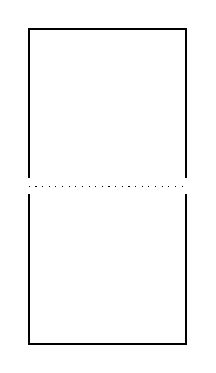
\begin{tikzpicture}[scale=2]    
    \draw[thick] (0,\eps)--(0,1)--(1,1)--(1,\eps);
    \draw[dotted] (0,0) -- (1,0);
    \draw[thick] (0,-\eps)--(0,-1)--(1,-1)--(1,-\eps);
\end{tikzpicture}
\caption{Staples}
\end{figure}


\begin{figure}
\centering
\begin{tikzpicture}
\begin{axis}[
    xlabel=$x$, ylabel=$y$,
    xmin=0, xmax=2*pi,
    ymin=0, ymax=10
]
\addplot[blue, domain=0:2*pi, samples=1000] {exp(2*cos(deg(x-1))};
\addplot[red, domain = 0:2*pi, dashed] {exp(2)};
\end{axis}
\fill[green] (1,2) circle (0.1);
\fill[red] (3,3) circle (0.1);
\end{tikzpicture}   
\caption{Accept-reject method. We accept the pair represented by the green dot, and reject the red one.}
\end{figure}

\section{Comparison of the Glauber and Heatbath algorithms for the Ising Model}

For the Ising model, the probability distribution of the Heatbath algorithm becomes
\begin{equation}
	p \propto \exp(-\beta s_x\Sigma_x),
\end{equation}
where $\Sigma_x$ is the sum of the nearest neighbors of the spin in site $x$. This is a discrete distibution in $s_x$ since there are only two posibilities for the spin: the proposal spin can be parallel to the original spin or it can be antiparallel. Therefore, the normalization constant is the sum of these possibilites, then
\begin{equation}
	p = \frac{\exp(-\beta s_x\Sigma_x)}{\exp(-\beta s_x\Sigma_x) + \exp(+\beta s_x\Sigma_x)}.
\end{equation} 
This can be rearrange to
\begin{equation}
	p = \frac{1}{1 + \exp(-2\beta s_x\Sigma_x)} = \frac{1}{1 + \exp(\Delta E)},
\end{equation}
which is the same as the Glauber probability.
\end{document}